\chapter{Introduction}
\label{chap:introduction}
%Here I will write my introduction. Needs a proper "målbeskrivelse"!
Low clouds have a net warming effect in the Arctic~\citep{Intrieri2002a}, as opposed to the well known net cooling effect they have at lower latitudes. Low layered clouds (stratus) also dominate the Arctic cloud cover. The Arctic climate changes have been greater than the global mean and have become known by the term "Arctic amplification"~\citep{Graversen2008}. Therefore the climate effect of low clouds in the Arctic is an interesting topic to study.

Decreasing sea ice extent could lead to an increase in the aerosol number concentrations in the area where ice has retreated. The open sea surface it self would lead to an increase in release of sea salt and DMS (dimethyl sulfide) to the lower atmosphere. The lack of sea ice would also increase the likelihood that the sea could be used for shipping, which would pollute the area.

The enhancement of evaporation from diminishing sea ice and the increase in aerosol number concentration from open water and shipping could lead to denser and longer-lived low clouds in the area of sea ice retreat. A followup question to that is if these clouds would then have a slightly different radiative effect, and by that influence the further retreat of sea ice.


%TEORI??@This warming is due the emission of longwave radiation that reaches the surface. At lower latitudes the clouds ability to reflect shortwave radiation would have a large enough cooling effect for the longwave emissions to be overpowered. In the Arctic the polar night in winter and high zenith angles in summer reduce the available shortwave radiation to reflect drastically, and the emission of longwave radiation outweighs the cooling effect by reflecting the shortwave radiation.
 

%\textbf{Must rewrite: Aside from producing precipitation, clouds have a profound effect on our climate. If you consider the overall effect of all clouds on the surface temperature, they have a cooling effect because they block incoming solar radiation. However, the effect of an individual cloud depends on many factors such as its height, thickness, location, and whether it is day or night. .... tatt fra nettet, Colorado State, CMMAP}. Througout this thesis shortwave (SW) radiation means solar radiation and longwave (LW) radiation covers the terrestrial infrared radiation.

\section{Main goal}
According to the IPCC report by~\citet{Boucher2013} the study by~\citet{Eastman2010b} using visual cloud reports from the Arctic, with surface and satellite observations, and the studies by~\citet{Kay2009} and~\citet{Palm2010} using lidar and radar observations have confirmed that the low-cloud amount over the Arctic oceans varies inversely with sea ice amount. This means that there is an increase in cloud amount when there is less sea ice. Now what we want to know is if these clouds are also denser and more persistent, and could lead to an enhanced warming and reduced sea ice amount, a positive feedback.

With this thesis I try to find if a decrease in Arctic sea ice lead to denser and more persistent clouds. It has been suggested that the decline in sea ice extent would allow for more pollution in the Arctic, as a consequence of more open water and ship traffic. The effect of increase in aerosol concentrations from shipping and open water, and the effect of enhanced evaporation from open water are studied separately and combined. With the main goal to find if this would lead to changes in clouds that could enhance downwelling long wave radiation and decrease upwelling short wave radiation, both of which have warming effects.

%(Something citing the IPCC report 2013 on the ice conditions in the Arctic, and something about Arctic clouds and radiation?)

\section{My contribution}
The findings in my thesis have been achieved with some of the most recently developed code (by Greg Thompson~\citep{Thompson2014}) for cloud micro physics and aerosols and their effects on radiation, in modeling. The results build further on the work of other researchers @name-some-and-cite and may raise some questions for further research within the field.

\section{Area description}
The area of the study in this thesis is in the Arctic, north of the United States of America and north-west of Canada. The study area covers the Beaufort Sea and a small part of Alaska and Canada, and can be seen in figure~\ref{fig:area}.

\begin{figure}
\centering
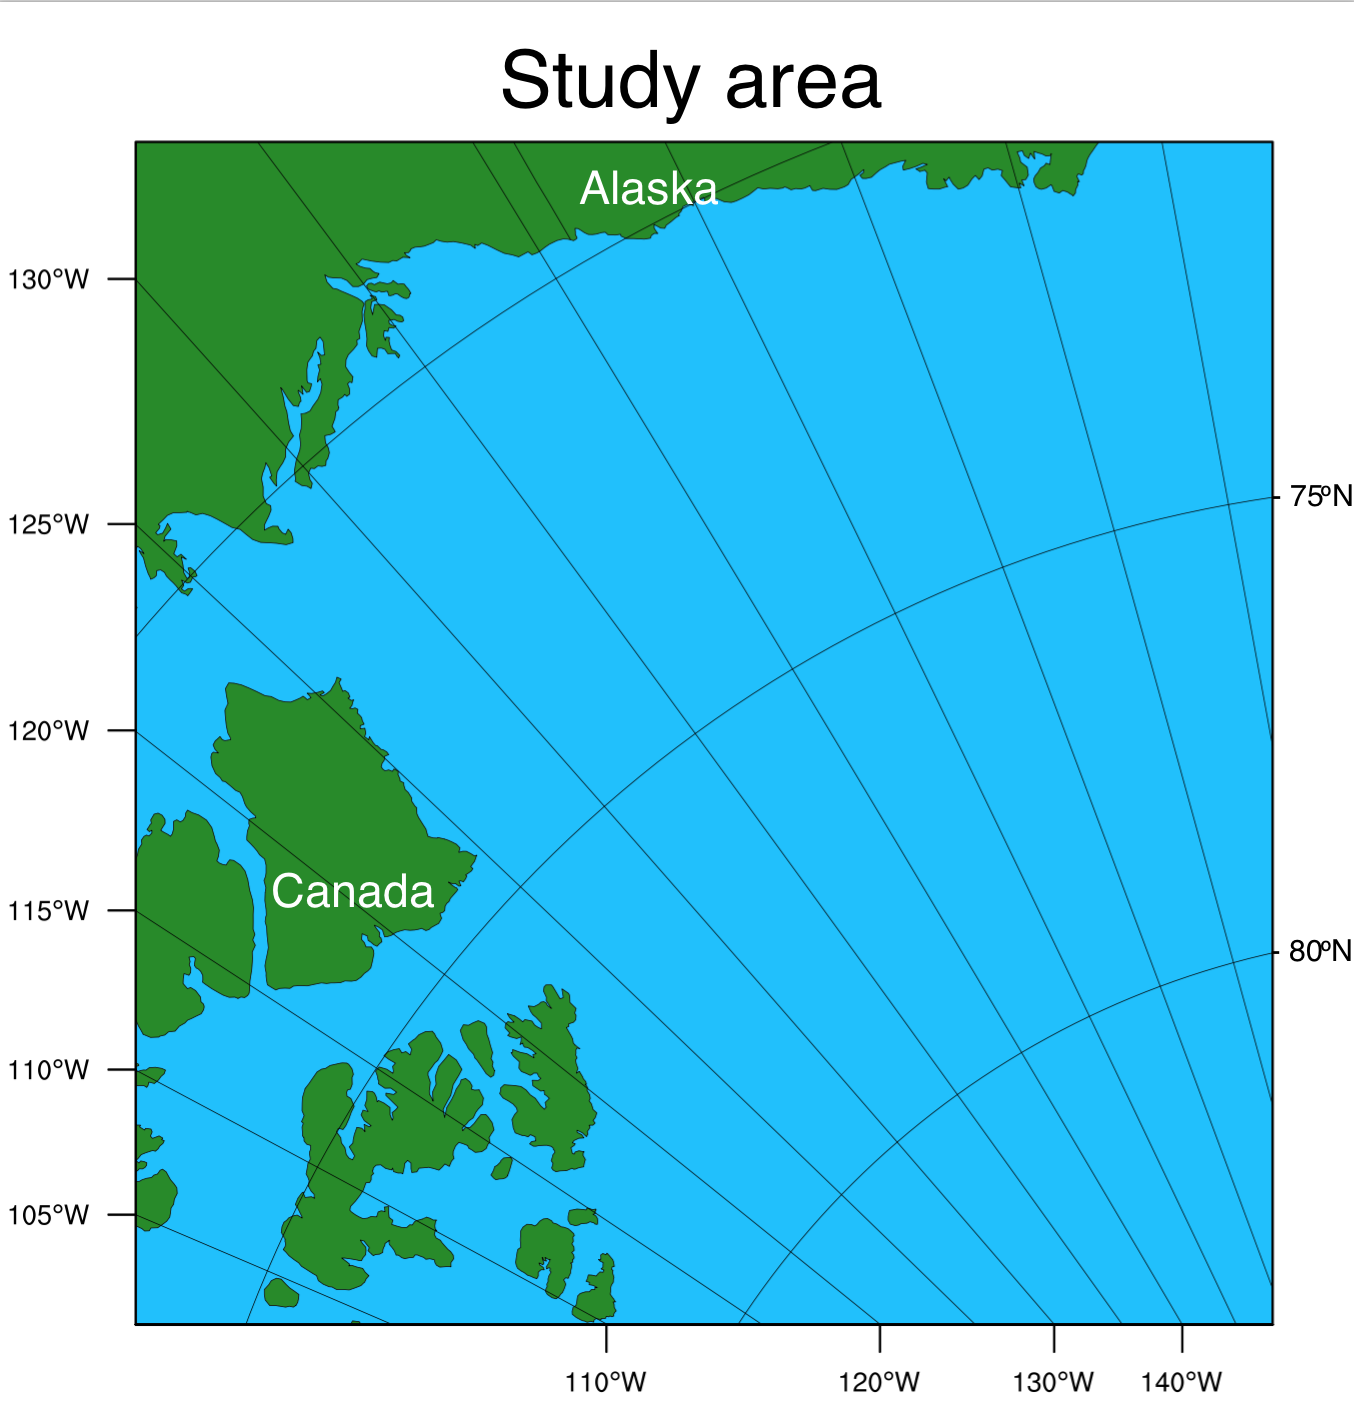
\includegraphics[width=0.7\textwidth]{introduction/studyarea.png}
\caption{An overview of the study area. The bottom right corner is the northernmost point and the y-axes show longitude and latitude to the left and right, respectivly.}
\label{fig:area}
\end{figure}
 
There are a few reasons for choosing this as the study area. First it is in the Arctic, and sea ice is present there in autumn, even in 2012 when there was record low sea ice extent. Also it has been exposed to field campaigns: Surface Heat Budget of the Arctic Ocean (SHEBA)~\citep{Uttal2002}, First International Satellite Cloud Climatology Project Regional Experiment Arctic cloud Experiment (FIRE ACE)~\citep{Curry2000}, Mixed-Phase Arctic Cloud Experiment (M-PACE)~\citep{Verlinde2007} and more. Therefore there are many studies on Arctic clouds that include this study area and data from some of the mentioned field campaigns. This provides parts of the science basis for my study and selection of literature and studies for comparison and questions. Quite a few studies are based on satellite data analysis and some of them are presented in the next chapter as background and motivation for my thesis.

\section{Structure of the thesis}
In the following chapter~\ref{chap:background} I will present the background for my thesis; what work I hope to compare my results to and relate my thesis to. Also I will touch upon why the subject of my thesis is important. In chapter~\ref{chap:theory} the most important theory and basic knowledge needed to understand some of the processes in clouds and their possible effect on the sea ice. Chapter~\ref{chap:modmet} is where I explain which model and tools and I have used and how I have worked with them to get the results presented and discussed in chapter~\ref{chap:results}.% The results are further discussed in chapter~\ref{chap:discussion}.
 A summary of main findings and conclusions are presented in the last chapter~\ref{chap:summaryconclusions}, before the list of references at the very end.


